\section{Security}
    Con il termine sicurezza informatica si intende quel ramo dell'informatica che si occupa dell'analisi delle vulnerabilità, del rischio, delle minacce e della successiva protezione dell'integrità logico-funzionale.

    La gran parte delle minacce derivano dalla rete Internet, per cui la sicurezza informatica è un tema importante nello studio delle reti di calcolatori.

    \begin{center}
        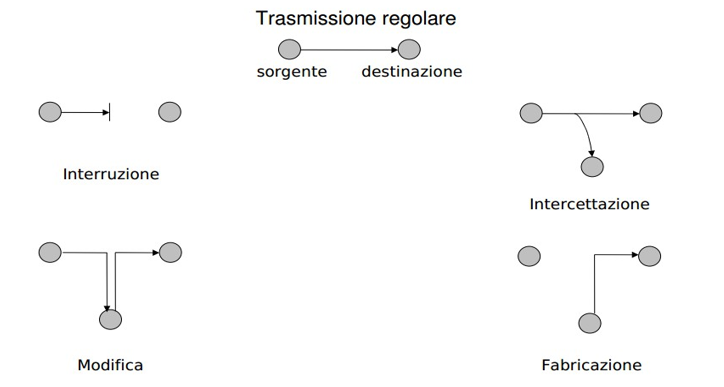
\includegraphics[scale=0.4]{chapters/7/assets/schema_a.png}
    \end{center}

    La realizzazione di un sistema che garantisca una assoluta protezione da abusi è impossibile, ma è possibile attivare meccanismi di sicurezza tali da limitare e scoraggiare i tentativi.

    La politica di sicurezza è quindi un compromesso, dettato dalle proprie necessità, tra il costo per attivarla ed il beneficio ottenuto in termini di diminuzione del rischio.

        \subsubsection{Security services}
            Per proteggere un host in rete o una comunicazione occorre stabilire dei servizi di sicurezza che possono essere classificati nel seguente modo:
            \begin{itemize}
                \item \textbf{Authentication}: un servizio che consente di accertare l'identità dichiarata da una entità (origine dei dati o peer in una comunicazione) mediate la verifica di credenziali.
                Avviene in due step: identificazione e verifica.
                \item \textbf{Authorization, Access Control}: protegge l'accesso ad una risorsa mediante l'applicazione di "Security Policy".
                \item \textbf{Confidentiality}: impedisce l'utilizzo delle informazioni da accessi non autorizzati.
                \item \textbf{Data Integrity}: consente di garantire che i dati acceduti non sono stati modificati.
                \item \textbf{System Integrity}: protegge le risorse del sistema contro modifiche, distruzioni accidentali o non autorizzate.
                \item \textbf{Non-Repudiation}: fornisce protezione contro il ripudio nel coinvolgimento in una comunicazione:
                \begin{itemize}
                    \item non ripudio della sorgente: prova chi è il mittente dei dati in una transazione.
                    \item non ripudio della destinazione: prova che i dati sono arrivati ad uno specifico destinatario.
                \end{itemize}
                \item \textbf{Avaliability}: fornisce una protezione per garantire accessibilità di una risorsa di sistema o di rete.
                \item \textbf{Audit (Accoutability, Traceability)}: registrazione di eventi di sistema o di rete. Consente di rintracciare, ricostruire (ed eventualmente addebitare) l'utilizzo delle risorse.
            \end{itemize}

    \subsection{Metodi di attacco}
        Esistono due tipologie di attacchi:
        \begin{itemize}
            \item \textbf{Attacco passivo}:
            \begin{itemize}
                \item raccolta di informazioni su possibili obiettivi (\textbf{confidentialy attacks}: network monitor, port scanning, etc.)
                \item intercettazione delle comunicazioni: eavesdropping, sniffing, etc.
            \end{itemize}
            \item \textbf{Attacco attivo}:
            \begin{itemize}
                \item fabbricazione dell'indentità di un'altra persona (authentication attacks): spoofing
                \item interruzione / compromissione di servizi (avaliability attacks): denial of service (DoS), Distributed DoS (DDoS)
                \item sfruttamento di bugs nel software installato (system integrity and authentication attacks): applicazione di exploit noti
                \item diffusione di vulnerabilità (system integrity attacks: virus, worms, bot, trojan
                \item ingegneria sociale: phishing.
            \end{itemize}
        \end{itemize}

        \subsubsection{Strumenti di attacco e difesa: sniffer e scanner}
            Uno sniffer analizza il traffico di rete utilizzando un analizzatore di protocollo è necessario un accesso privilegiato all'interfaccia di rete, possono essere orientati ad analizzare una sequenza di pacchetti (es. \verb|tcpdump| e \verb|wireshark|).
        
            Uno scanner cerca di connettersi ad un intervallo di numeri di porta o indirizzi IP per vedere quali servizi o sistemi sono presenti ed attivi.
        
            Un esempio è \verb|nmap|: uno strumento open-source per la network exploration e l'auditing.
        
            Opzioni significative del comando:
            \begin{itemize}
                \item \verb|-sP| (ping scan)
                \item \verb|-sT| (TCP connect() - default)
                \item \verb|-sS| (TCP syn, richiede i privilegi di root)
                \item \verb|-A| rileva versione
                \item \verb|-p| seleziona le porte da testare (es. \verb|nmap -A 192.168.0.254 -p 22 80| \verb|01-8060|)
            \end{itemize}

            Lo strumento \textbf{Network Monitor} analizza il traffico della rete, come ad esempio \verb|ntop|.

        \subsubsection{Strumenti di attacco: Spoofing (fabbricazione)}
            Uno \textbf{spoofing} è un tipo di attacco informatico dove viene impiegata la falsificazione dell'identità (spoof). Quando la falsificazione non avviene in campo informatico, si parla di \textbf{social engineering}.
        
            Si hanno diverse tipologie di spoofing:
            \begin{itemize}
                \item \textbf{User account spoofing}: usare nome utente e password di un altro utente senza averne il diritto. Può avvenire utilizzando strumenti come sniffer e password crackers. I password cracker possono essere off-line come John the ripper, oppure on-line, come Hydra e Medusa.
                \item \textbf{IP Address spoofing}: si basa sul fatto che la maggior parte dei routers all'interno di una rete, controllino solo l'indirizzo IP di destinazione e non quello sorgente. Le finalità di questo attacco sono superare le tecniche difensive basate sull'autenticazione dell'indirizzo e realizzare attacchi DDoS.
                \item \textbf{MAC Address forging}: il MAC address viene modificato impersonando l'indirizzo della vittima. Diversi sistemi di autenticazione/autorizzazione sono basati su MAC address quali aAutenticazione verso DHCP server e sessioni attive su Captive Portal (Session Hijacking).
                \item \textbf{ARP Spoofing / Poisoning}: consiste nell'inviare intenzionalmente de in modo forzato risposte ARP contenenti dati inesatti. In questo modo la tabella ARP di un host conterrà dati alterati. Ettercap è un tool per attacco di tipo man-in-the-middle, basato su ARP poisoning.
            \end{itemize}

        \subsubsection{Strumenti di attacco: Denial of Service (DoS)}
            I \textbf{Denial of Service (DoS)} causano la perdita dell'utilizzo di una risorsa sovraccaricandola, ma non ne permettono l'accesso all'attaccante.
        
            Gli attacchi possono essere diretti (l'attaccante interagisce direttamente con la vittima), oppure possono essere indiretti (l'attaccante sfrutta terze parti).
        
            I principali attacchi sono:
            \begin{itemize}
                \item \textbf{Flooding}:
                \begin{itemize}
                    \item \textit{Ping floods}: invio di ICMP echo request in numero maggiore a quelli gestibili dal sistema attaccato; l'aggressore invia un grosso flusso di traffico ICMP echo verso una serie di indirizzi di broadcast attribuendosi come indirizzo sorgente quello della vittima.
                    \item \textit{TCP SYN Floods}: funziona se un server alloca delle risorse dopo aver ricevuto un SYN, ma prima di aver ricevuto un messaggio ACK (vedi \verb|nmap -sS|).
                \end{itemize}
                \item \textbf{Invio di pacchetti malformati}:
                \begin{itemize}
                    \item \textit{Ping of death}: si inviano ping di grandi dimensioni che possono causare buffer overflow con conseguente blocco del servizio, o in casi più gravi, il crash del sistema.
                    \item \textit{UDP bombs}: sono costituiti con valori illegali in certi campi. In certi sistemi operativi la ricezione di pacchetti imprevisti ne può causare il crash.
                \end{itemize}
                \item \textbf{Attacchi da più host}:
                \begin{itemize}
                    \item DDoS: è una variante di DoS realizzato utilizzando numerose macchine che in insieme costituiscono una botnet controllate da un'unica entità, il botmaster.
                \end{itemize}
            \end{itemize}

        \subsubsection{Strumenti di attacco: exploit}
            Un \textbf{exploit} è un frammento di codice, una sequenza di comandi, o un insieme di dati, che prendono vantaggio da un bug o da una vulnerabilità per acquisire privilegi di accesso, eseguire codice o creare DoS su di una risorsa.
        
            I più comuni tipi di \textit{exploit} prendono vantaggio da:
            \begin{itemize}
                \item \textbf{Buffer overflow (stack o heap)}: si basa sul fatto che un programma potrebbe non controllare in anticipo la lunghezza dei dati in arrivo, ma si limita a scrivere il loro valore in un buffer di lunghezza prestabilita, confidando che l'utente (o il mittente) non immetta più dati di quanti esso ne possa contenere.
                \item \textbf{Code injection}: questo exploit sfrutta l'inefficienza dei controlli sui dati ricevuti in input ed inserisce codice maligno (ad esempio all'interno di una query SQL).
            \end{itemize}

            Spesso, quando gli exploit vengono pubblicati, la vulnerabilità viene eliminata attraverso una patch che produce una nuova versione del software.

        \subsubsection{Strumenti di attacco: malware}
            Un \textbf{malware} è un qualsiasi software creato allo scopo di causare danni ad un computer, ai dati degli utenti, o ad un sistema informatico su cui viene eseguito. Si indetificano in malware:
            \begin{itemize}
                \item \textbf{Virus}: sono parti di codice che si diffondono copiandosi all'interno di altri programmi, o in una particolare sezione del disco fisso, in modo da essere eseguiti ogni volta che il file infetto viene aperto.
                \item \textbf{Worm}: questi malware non hanno bisogno di infettare altri file per diffondersi, perché modificano il sistema operativo della macchina ospite in modo da essere eseguiti automaticamente e tentare di replicarsi sfruttando per lo più Internet.
                \item \textbf{Trojan}: software che oltre ad avere delle funzionalità "lecite", utili per indurre l'utente ad utilizzarli, contengono istruzioni dannose che vengono eseguite all'insaputa dell'utilizzatore.
                \item \textbf{Spyware}: software che vengono usati per raccogliere informazioni dal sistema su cui sono installati e per trasmetterle ad un destinatario interessato.
            \end{itemize}

        \subsubsection{Strumenti di attacco: ingegneria sociale e spam}
            L'\textbf{ingegneria sociale} è lo studio del comportamento individuale di una persona al fine di carpire informazioni utili. Ad esempio, il \textbf{phishing} è un tipo di ingegneria sociale attraverso la quale un aggressore cerca di ingannare la vittima convincendola a fornire informazioni personali sensibili.
        
            Lo \textbf{spamming} è l'invio di messaggi indesiderati (generalmente commerciali). Può essere attuato attraverso qualunque sistema di comunicazione, ma il più usato è Internet, attraverso messaggi di posta elettronica. L'80\% delle email inviate oggi nel mondo è spam.

        \subsubsection{CERT: Computer Emergency Response Team}
            Un \textbf{CERT} è un servizio offerto all'interno di una comunità di utenti Internet per la gestione di emergenze in seguito ad attacchi informatici.
        
            CERT rilevanti in Italia: \textbf{GARR}.

    \subsection{Strumenti di difesa}
        Gli strumenti di difesa possono essere:
        \begin{itemize}
            \item \textbf{Policy per l'utente e l'amministratore}:
            \begin{itemize}
                \item Password Policy (authentication).
                \item Antivirus/ Antispam (system integrity, availabilty).
                \item Aggiornamenti automatici (system integrity).
                \item Analisi dei Log (audit).
            \end{itemize}
            \item \textbf{Difesa della LAN o dell'host}:
            \begin{itemize}
                \item Firewall Packet filter e Firewall Proxy (system integrity).
                \item Sniffer e IDS (availability).
                \item Ethical Hacking.                
            \end{itemize}
            \item \textbf{Rinforzo di autenticazione e riservatezza, strumenti crittografici}:
            \begin{itemize}
                \item Tools: crittografia simmetrica e asimmetrica, Message Digest, certificati.
                \item Servizi: autenticazione (authentication), cifratura, (data confidentialy), firma digitale (data integrity).
            \end{itemize}
        \end{itemize}

        \subsubsection{Password Policy}
            La password è una delle forme di identificazione più semplici ed utilizzate ed è quindi uno dei principali bersagli degli attacchi.
        
            I metodi più utilizzati sono:
            \begin{enumerate}
                \item Intercettazione: l'utilizzo di un canale non cifrato consente la cattura delle password sulla rete.
                \item Furto: gli utenti tendo a scriverla su un supporto magnetico per non dimenticarla.
                \item Tentativi di indovinare la password(password cracker basati su dizionari).
                \item Phishing.
            \end{enumerate}

            Molte debolezze (2, 3 e 4) dipendono dal comportamento dell'utente, a cui viene richiesto di rispettare policy specifiche nella gestione della password. Ad esempio riguardo il punto 3: "la password dovrà essere lunga fra gli 8 e i 15 caratteri e contenere almeno un numero o un carattere fra questi \$\%\&(), una password non potrà essere riutilizzata prima di un anno dall'ultima volta che è stata impostata, una password non potrà contenere più di due caratteri consecutivi del nome utente".

        \subsubsection{Auditing: syslog, logrotate, logwatch}
            La gestione e l'analisi degli eventi di sistema e di rete consente l'early warning, ovvero individuare rapidamente eventuali attacchi in corso, e il trouble shooting, cioè mantenere uno storico degli eventi per tracciare attività.
        
            I principali strumenti sono:
            \begin{itemize}
                \item \textbf{syslog} (log sever), in cui vengono specificate facility (KERN, USER, MAIL, DEAMON, etc.), priorità (EMERG, ALERT, CRIT), azioni (scrivere su file, inviare email, attivare script, etc.).
                Nel file \verb|/etc/syslog.conf| vengono definite le azioni.

                I messaggi possono essere inviati tramite API:

                \verb|#include <syslog.h>|

                \verb|void openlog(const char* ident, int option, int facility);|

                \verb|void syslog(int priority, const char* format);|

                \verb|void closelog(void);|
                \item \textbf{logrotate}: per agevolare l'analisi dei log azzera i file con cadenza regolare (es: ogni giorno) e mantiene per un determinato periodo i vecchi file.

                Esempio di file \verb|/etc/logrotate.conf|:

                \verb|weekly # rotate log files weekly|

                \verb|rotate 4 # keep 4 weeks worth of backlog|
                
                \verb|compress|

                \verb|create # create new empty log file after rotating|
                \item \textbf{logwatch}: quando viene eseguito processa i file di log selezionati e invia una mail di report. I principali servizi monitorati (default) sono: dhcpd, httpd, named, connections, sshd, sudo, yum, disk space.
                
                logwatch ha dei limiti: se un intrusore fa in tempo a modificare i log e cancellare le sue tracce, logwatch non si accorge di nulla.
                
                Esempio di utilizzo:

                \verb|logwatch -print -detail High -archives -range All|
            \end{itemize}

    \subsection{Firewall}
        Per \textbf{firewall} si intende un'entità hardware o software che si pone tra internet e la rete (LAN firewall) o host (personal firewall) che si vuole proteggere.
    
        Il firewall svolge una funzione di filtro, consentendo il transito solamente alle connessioni ritenute lecite mediante una opportuna \textbf{policy}.
    
        Gli obbiettivi principali sono quelli di monitorare, limitare, autenticare l'accesso alla rete da proteggere nei confronti di accessi provenienti dall'esterno (Internet) e quello di monitorare, limitare, autenticare l'accesso all'esterno (Internet) da parte dell'utenza interna.

        \begin{center}
            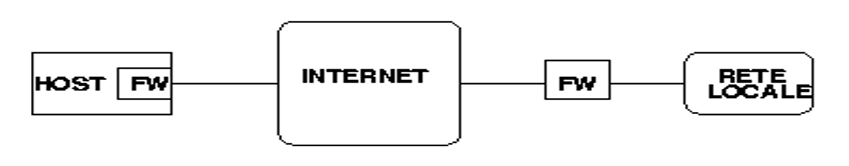
\includegraphics[scale=0.4]{chapters/7/assets/schema_b.png}
        \end{center}

        I firewall possono essere di due tipi:
        \begin{itemize}
            \item \textbf{packet filter}: agiscono ai livelli network e transport.
            \item \textbf{proxy}: agiscono a livello applicazione.
        \end{itemize}

        \subsubsection{Firewall a filtro di pacchetti}
            Questo filtro analizza tutti i pacchetti in transito e applica azioni del tipo permit/deny sulla base di politiche basate sugli indirizzi IP e le porte di provenienza e/o di destinazione.
        
            Gli obiettivi sono quelli di rendere visibili ad internet solamente i servizi di rete destinati ad un accesso pubblico (protezione dei servizi intranet e dei servizi "inconsapevoli"); bloccare il traffico indesiderato (es: P2P), e fare da strumento per la gestione delle emergenze (bloccare un host ostile o contaminato da virus).
        
            Agisce a livello di pacchetti IP, ma deve leggere anche i primi byte del livello transport per leggere le porte TCP o UDP.
        
            Può essere realizzato dai router mediante un modulo aggiuntivo o da HW specifico.
        
            Per Linux esiste il modulo \textbf{IPtables} che può essere applicato ad una interfaccia di rete.

        \subsubsection{ACL sul router}
            Il router è un apparato di rete posto solitamente tra LAN e Internet, che svolge il compito di gestione dei singoli pacchetti per il loro instradamento. La gran parte dei router possono essere configurati per svolgere anche la funzionalità di packet filter.

            Il sistema operativo IOS dei router Cisco consente la definizione di \textbf{ACL (Access Control List)} che possono essere applicate alle interfacce del router.
        
            In questo esempio viene creata una ACL sul traffico entrante che consente l'accesso ai soli server web ed e-mail, bloccando il resto. L'ACL è poi applicata all'interfaccia opportuna:

            \verbatiminput{chapters/7/assets/schema_c.h}

        \subsubsection{IPtables}
            Il pacchetto software \textbf{IPtables} consente di applicare ACL per il packet filtering sulle interfacce dei sistemi Linux. IPtables lavora sulle 3 tabelle filter, nat, mangle sulle quali possiamo creare catene (chains) di regole ACL.
        
            La \textbf{tabella filter} (tabella di default) serve per il packet filter.
            Le tabelle \textbf{NAT (SNAT e DNAT)} servono per le regole di NATting. La \textbf{tabella mangle} serve per modificare alcuni parametri nell'header pacchetto. La \textit{tabella filter} ha 3 catene di default applicate su una sola interfaccia di rete:
            \begin{itemize}
                \item \textbf{Input}: per il processamento dei pacchetti destinati all'host.
                \item \textbf{Output}: per i pacchetti provenienti dall'host.
                \item \textbf{Forward}: per i pacchetti che devono attraversare il firewall.
            \end{itemize}

            \begin{center}
                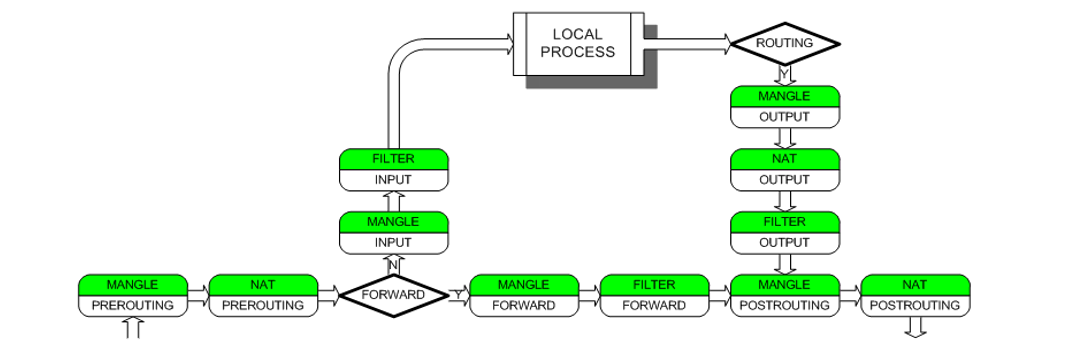
\includegraphics[scale=0.32]{chapters/7/assets/schema_d.png}
            \end{center}

            \subsubsection*{Esempi di IPtables}

            \verbatiminput{chapters/7/assets/schema_e.sh}

        \subsubsection{Firewall basati su proxy}
            Il \textbf{proxy} è un programma applicativo con funzione di tramite tra client e server. In modo implicito o esplicito il client deve rivolgersi al \textit{proxy} per poter raggiungere il server. Occorre un Proxy specifico per ogni applicazione.
        
            Gli obbiettivi del proxy sono: mettere in comunicazione client e server che non hanno visibilità diretta (ad esempio se il client è in una intranet), migliorare le prestazioni (es: web caching), aggiungere funzionalità di security (monitoraggio, autenticazione, filtro).
        
            Esempi di proxy sono: proxy web (squid) e proxy SMTP (virus e spam scanners, etc.).

            \begin{center}
                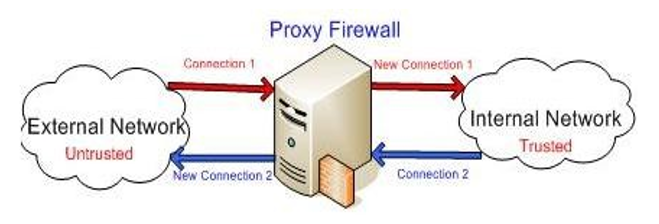
\includegraphics[scale=0.5]{chapters/7/assets/schema_f.png}
            \end{center}

    \subsection{IDS}
        L'\textbf{IDS (Intrusion Detection System)} è un dispositivo software/hardware per identificare accessi non autorizzati a host o LAN.
    
        L'IDS generalmente si appoggia su un database per memorizzare le regole utilizzate per individuare le violazioni di sicurezza.
    
        Gli IDS sono classificabili nel seguente modo:
        \begin{itemize}
            \item \textbf{Host IDS (HIDS)}: analizzano file di log e file system sull'host. TRIPWIRE è un esempio di HIDS. Si basa sulla differenza tra lo stato analizzato ed uno stato iniziale.
            \item \textbf{Network IDS (NIDS)}: analizzano il traffico di rete.
            SNORT è un esempio di NIDS che può funzionare anche come sniffer o packet logger.
            \item \textbf{Ibridi}: svolgono entrambe le funzioni.
        \end{itemize}
    
    \subsection{IPS}
        Gli \textbf{IPS (Intrusion Prevention Systems)} sono un'estensione degli strumenti di IDS: a differenza dai componenti IDS, sono posizionati on-line e sono abilitati a prevenire e bloccare le intrusioni identificate.
    
        IPS può eseguire alcune azioni come mandare un allarme, eliminare pacchetti malevoli, resettare le connessioni e/o bloccare il traffico da un indirizzo IP attaccante.
    
        Fail2ban è pensato per prevenire attacchi brute force, bloccando temporaneamente gli indirizzi IP che provano a violare la sicurezza di un sistema.
    
    \subsection{Antivirus}
        L'\textbf{Antivirus (AV)} è un software atto a prevenire, rilevare ed eventualmente eliminare programmi dannosi. Un AV ha anche una funzione preventiva, impedendo che un virus possa entrare in un sistema ed infettarlo.
    
        Il metodo più utilizzato per individuare virus in un file è attraverso le signatures (firme). Il programma AV calcola la firma (signature) di un file da analizzare (es: Hash MD5 dell'intero file) e lo confronta con le firme di virus noti presenti all'interno di un archivio. Se la firma corrisponde il file è sicuramente un virus.
    
        Esistono anche tecniche euristiche, di solito usate in modo complementare alle firme, che cercano di individuare virus non noti all'AV attraverso la ricerca di pattern sospetti.
    
        Può essere installato sul PC, scan dei dischi dell'host e dei nuovi file salvati, oppure sul mail server, scan delle mail in entrata ed in uscita.

    \subsection{Tecniche antispam}
        Esiste una lista di server classificati spammersm, che viene attivata sul mail server rifiutando mail che provengono da questa lista. L'amministratore del mailserver può costruire manualmente una propria lista o può avvalersi di servizi in Internet che distribuiscono automaticamente le liste.
    
        \textbf{Gray-List}: si basano sul fatto che i mailer usati dagli spammer generalmente tentano l'invio di una email una sola volta, il Graylisting consiste nel rigetto della ricezione della mail al primo tentativo, che verrà accettata ad un successivo tentativo, dopo un tempo stabilito (tipicamente 300 secondi).
    
        \textbf{White List}: liste di mittenti fidati, su cui non vengono effettuati controlli antispam. Include gli host accettati da Gray-list e host inseriti manualmente dall'amministratore.
    
        \textbf{Filtri Bayesiani}: sono filtri che cercano di classificare le mail in arrivo assegnando un punteggio numerico a frasi o modelli che si presentano nel messaggio. Ogni messaggio riceve quindi un punteggio compressivo (tra 0 e 1) che, dopo aver stabilito una soglia, consente di classificare il messaggio. Il filtro richiede un addestramento con mail spam e no-spam con cui viene creato un database di riferimento.
    
        Esempi di antispam sono Spamassassin (basato su liste white e black e filtri Bayesiani) e Bogofilter (basato su filtri Bayesiani).
    
    \subsection{Crittografia}
        La \textbf{crittografia} è lo studio dei metodi per rendere un messaggio ofuscato in modo da renderlo comprensibile solo a persone a cui il messaggio è destinato (servizio di sicurezza Confidenzialità).
    
        L'algoritmo che esegue la cifratura o decifratura è detto \textbf{cipher}.
    
        La \textbf{cifratura E (encryption)} si applica ad un \textbf{messaggio in chiaro P (plaintext)} per ottenere un testo cifrato \textbf{C (ciphertext)}.

        \begin{equation*}
            C = E(P)
        \end{equation*}

        La \textbf{decifratura D (decryption)} si applica ad un messaggio cifrato C per ottenere il testo in chiaro P.

        \begin{equation*}
            P = D(C)
        \end{equation*}

        I \textit{cipher} sono parametrizzati da una chiave segreta $k$.

        Se gli algoritmi utilizzano la stessa chiave per cifrare e decifrare sono detti a chiave simmetrica, altrimenti sono detti a chiave pubblica.

        A chiave simmetrica:

        \begin{equation*}
            C = E(P,k) P = D(C,k)
        \end{equation*}

        A chiave pubblica:

        \begin{equation*}
            P = D(C,k_2) c = E(P,k_1)
        \end{equation*}

        La \textbf{crittanalisi} è lo studio dei metodi per ottenere il significato di un testo cifrato, violando la tecnica di cifratura per verificarne la robustezza. Tipicamente si tratta di trovare una chiave segreta.

        \begin{center}
            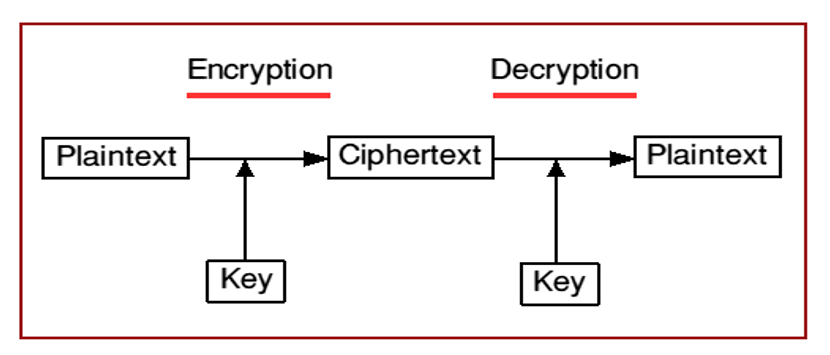
\includegraphics[scale=0.38]{chapters/7/assets/schema_g.png}
        \end{center}

        \subsubsection{Crittografia nelle reti}
            Gli algoritmi crittografici simmetrici e gli algoritmi a chiave pubblica vengono utilizzati per costruire protocolli di rete con l'obiettivo di cifrare la comunicazione, fornendo diversi servizi di sicurezza quali la Confidenzialità, l'Autenticazione e il Non Ripudio.
        
            Il principale protocollo di questo tipo è \textbf{SSL (Secure Socket Layer)}, poi diventato \textbf{TLS (Transport Security Layer)}.
        
            SSL o TLS è strutturato come un layer che si pone tra il trasporto (TCP) e l'applicazione. Molte applicazioni di rete (ad esempio HTTP, IMAP, LDAP) sono state adattate per appoggiarsi su SSL (anziché TCP) per usufruire dei servizi di sicurezza del protocollo.

            \begin{center}
    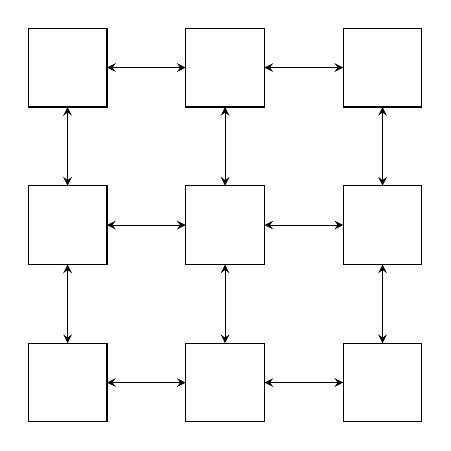
\begin{tikzpicture}
        %%%%%%%%%% Nodi %%%%%%%%%%
        \draw (0,0) rectangle (1,1);
        \draw (2,0) rectangle (3,1);
        \draw (4,0) rectangle (5,1);
        \draw (0,2) rectangle (1,3);
        \draw (2,2) rectangle (3,3);
        \draw (4,2) rectangle (5,3);
        \draw (0,4) rectangle (1,5);
        \draw (2,4) rectangle (3,5);
        \draw (4,4) rectangle (5,5);

        %%%%%%%%% Frecce %%%%%%%%%
        \draw[<->,>=stealth] (1,0.5) -- (2,0.5);
        \draw[<->,>=stealth] (3,0.5) -- (4,0.5);
        \draw[<->,>=stealth] (1,2.5) -- (2,2.5);
        \draw[<->,>=stealth] (3,2.5) -- (4,2.5);
        \draw[<->,>=stealth] (1,4.5) -- (2,4.5);
        \draw[<->,>=stealth] (3,4.5) -- (4,4.5);
        \draw[<->,>=stealth] (0.5,1) -- (0.5,2);
        \draw[<->,>=stealth] (2.5,1) -- (2.5,2);
        \draw[<->,>=stealth] (4.5,1) -- (4.5,2);
        \draw[<->,>=stealth] (0.5,3) -- (0.5,4);
        \draw[<->,>=stealth] (2.5,3) -- (2.5,4);
        \draw[<->,>=stealth] (4.5,3) -- (4.5,4);
    \end{tikzpicture}
\end{center}

            \begin{center}
                HTTP + SSL/TLS + TCP = HTTPS
            \end{center}

        \subsubsection{SSL e TLS}
            \textbf{SSL (Secure Socket Layer)} è un protocollo sviluppato originariamente dalla Netscape per fornire autenticazione e privacy in una connessione tra client ed un server l'uso di diverse tecnologie crittografiche.
        
            Le principali tecnologie sono:
            \begin{itemize}
                \item Algoritmi crittografici (a chiave simmetrica o pubblica)
                \item Message Digest (firma digitale)
                \item Certificati e Certification Authority
                \item SSL e TLS
            \end{itemize}

            Le implementazioni SSL e TLS sono:
            \begin{itemize}
                \item \textbf{OpenSSL}: è una libreria open source basata sulla libreria SSLeay con una licenza specifica più restrittiva ed incompatibile rispetto a GPL. Utilizza i protocolli SSLv2 SSLv3 e TLSv1.
                
                Utilizza algoritmi cipher simmetrici, crittografia a chiave pubblica, certificati, hash, etc.
                
                Fornisce un \textbf{ToolKit} per l'utilizzo a linea di comando delle API, una \textbf{libreria SSL} per la programmazione di canali cifrati SSL/TLS, la \textbf{libreria Crypto} per la programmazione di diversi algoritmi crittografici tra cui la cifratura a chiave simmetrica, a chiave pubblica, certificati e funzioni di Hash.
                \item \textbf{GnuTLS}: creato per consentire alle applicazioni del progetto GNU di usare una libreria TLS compatibili con GPL. Ha licenza GPL e LGPL.
                
                Utilizza protocolli SSLv3.0, TLSv1.0, TLSv1.1, TLSv1.2, DTLS 1.2.

                Fornisce API di programmazione (C/C++, Python) ed alcune utilities di supporto.
            \end{itemize}

        \subsubsection{OpenSSL ToolKit}
            Il ToolKit consente l'utilizzo a linea di comando di tutte le operazioni crittografiche della libreria.

            Principali comandi:
            \begin{itemize}
                \item \textbf{Cipher simmetrici}: \verb|enc| (base64, bf, des, des3, idea, rc4, rc5).
                \item \textbf{Crittografia a chiave pubblica}: \verb|x.509| (gestione dati dei certificati), \verb|ca| (per utilizzare le funzioni di Ceritification Authority), \verb|req| (richiesta di certificati), \verb|verify| (verifica di certificati), \verb|crl| (Certificate Revocation List), \verb|crl2pkcs7 pkcs7|(conversione tra diversi formati di certificati).
                \item \textbf{Message digest}: \verb|dgst| (md2, md5, rmd160, sha, sha1).
                \item \textbf{Altro}: \verb|ciphers -v| (elenco ciphers supportati), \verb|speed| (benchmarking), \verb|prime| (numeri primi) e \verb|rand|, \verb|password|, \verb|smime|, \verb|s_client|, \verb|s_server|.
            \end{itemize}
            
        \subsubsection{Comandi OpenSSL: base64}
            Viene utilizzata per codificare una sequenza binaria in una sequenza di caratteri ASCII.
        
            La sequenza binaria è suddivisa in blocchi di 6 bit, ciascuno dei quali viene trasformato in un carattere ASCII mediante un alfabeto di 64 caratteri [a-z, A-Z, 0-9./]

            \verbatiminput{chapters/7/assets/schema_i.sh}

        \subsubsection{Comandi OpenSSL: prime e rand}
            OpenSSL contiene routine per trattare numeri primi e numeri random (poiché questi servono per le tecniche crittografiche).

            \verbatiminput{chapters/7/assets/schema_j.sh}

        \subsubsection{Crittografia a chiave simmetrica}
            È una tecnica crittografica a chiave condivisa che consente di ottenere la cifratura di un messaggio $P$, $C = E_K (P)$ in modo che la stessa chiave possa essere utilizzata per decifrarlo $P = D_K(C)$.

            Gli algoritmi $E$ e $D$ (cipher) sono noti. La complessità della cifratura è data da $K$ la cui lunghezza determina l'ampiezza dello spazio delle possibili codifiche di $P$, di conseguenza, la robustezza della cifratura.

            \begin{center}
                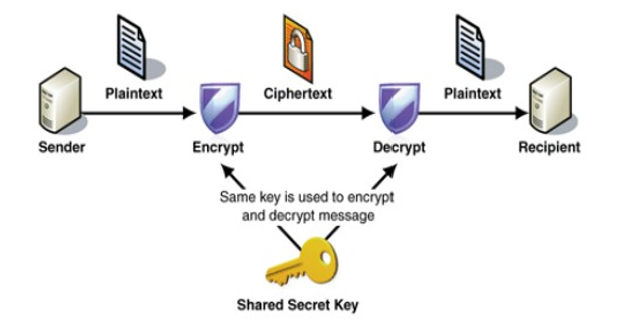
\includegraphics[scale=0.5]{chapters/7/assets/schema_k.png}
            \end{center}

            Le applicazioni principali sono: attivazione di una comunicazione su un canale insicuro, e la cifratura delle password.

        \subsubsection{Cipher simmetrici}
            OpenSSL supporta tutti i principali cipher simmetrici, tra cui:
            \begin{itemize}
                \item \textbf{DES (Data Encryption Standard)}: sviluppato da IBM, lavora su blocchi del messaggio di 64 bit, con chiave di 64 bit di cui 8 sono di parità dispari, pertanto la chiave è di 56 bit.
                
                La lunghezza della chiave è troppo breve e l'algoritmo può essere forzato in poche ore.
                \item \textbf{TripleDES}: è l'algoritmo DES applicato tre volte. Può utilizzare 1,2 o 3 chiavi DES.
                \item \textbf{AES (Advanced Encryption Standard)}: l'algoritmo supporta chiavi da 128, 192, o 256 bit su blocchi da 128 bit.
                \item \textbf{RC4} è un algoritmo a 128 bit utilizzato nei protocolli quali SSL e WEP (WiFi).
            \end{itemize}

        \subsubsection{Comandi OpenSSL: enc}
            Questo comando serve per cifrare/decifrare utilizzando uno tra i cipher simmetrici supportati che sono circa 50, tra cui: \verb|-des|, \verb|-des3|, \verb|-aes128|, \verb|-aes192|, \verb|-aes256|, \verb|-rc4|.

            \verbatiminput{chapters/7/assets/schema_l.sh}

        \subsubsection{Message Digest}
            Il \textbf{Message Digest (MD)} è una sequenza di bit di lunghezza limitata e fissa associata ad un messaggio (P) e cne rappresenta la firma (o impronta).
        
            Il MD non è invertibile, ovvero non è possibile risalire al messaggio originale. Se il messaggio cambia anche di un solo bit, il MD diventa completamente diverso.
        
            Il MD viene calcolato applicando al messaggio una funzione di hash:

            \begin{equation*}
                MD = H(P)
            \end{equation*}

            L'algoritmo deve essere \textbf{Collision Free}, ovvero deve evitare (o minimizzare) la possibilità che due messaggi generino lo stesso $MD$. Per questo motivo il $MD$ non può essere troppo breve.

            Le applicazioni principali del $MD$ sono la verifica dell'integrità di messaggi o di file: il messaggio $P$ viene spedito assieme al $MD$, chi li riceve ricalcola i $MD$ e lo compara con quello ricevuto e per la verifica della password: viene memorizzato il $MD$ della password in chiaro $MD = H(clear passw)$. Per verificare la password bisogna confrontare $H(proposed clear passw)$ con $MD$.

        \subsubsection{Comandi OpenSLL: dgst}
            I principali digest sono:
            \begin{itemize}
                \item \textbf{MD5}: è un'algoritmo di hashing a 128 bit realizzato nel 1991.
                \item \textbf{RIPEMD}: è una famiglia di algoritmi sviluppati come alternativa a MD5, il più importante è \textbf{ripemd160}.
                \item \textbf{SHA (Sechure Hash Algorithm)}: indica una famiglia di 5 diverse funzioni, sviluppate da NSA come standard federale del governo USA. Esistono varie versioni: sha1 (160 bit), sha2 (sha224 (224 bit), sha256 (256 bit), sha384 (384 bit), sha512 (512 bit)).
            \end{itemize}

            Il comando \verb|dgst| serve ad applicare una tra le funzioni di hash supportate:

            \verbatiminput{chapters/7/assets/schema_m.sh}

        \subsubsection{HMAC}
            Se due parti A e B condividono una chiave simmetrica, possono autenticare i messaggi che si scambiano utilizzando lo schema \textbf{HMAC (Hashed Message Authentication Code)} che è una funzione di hash applicata al messaggio e alla chiave condivisa:
            
            \begin{equation*}
                Firma = HMAC(K,M)
            \end{equation*}

            Il mittente che deve inviare M calcola $HMAC(K,M)$ che invia assieme ad $M$; il destinatario riceve $M$ e $HMAC(K,M)$, quindi verifica la firma ricalcolando l'HMAC.

            Questo schema è utilizzato in diversi protocolli crittografici, tra cui IPsec.

            \verbatiminput{chapters/7/assets/schema_n.sh}

        \subsubsection{Password}
            La password è una sequenza alfanumerica che l'utente deve inserire per accedere ad una risorsa protetta. È quindi un segreto condiviso tra utente e risorsa, che normalmente la risorsa memorizza in formato cifrato.
        
            La cifratura non è invertibile, quindi per la verifica occorre cifrare la password da verificare e confrontarla con la password cifrata memorizzata dalla risorsa. La cifratura avviene utilizzando cipher simmetrici, o funzioni di Hash. Spesso si utilizza usa stinga casuale, detta \textbf{salt}, per complicare gli attacchi al dizionario.
        
            Il comando \verb|passwd| per generare le password Unix/Linux si basa sulla funzione \verb|crypt()|.
        
            \begin{center}
                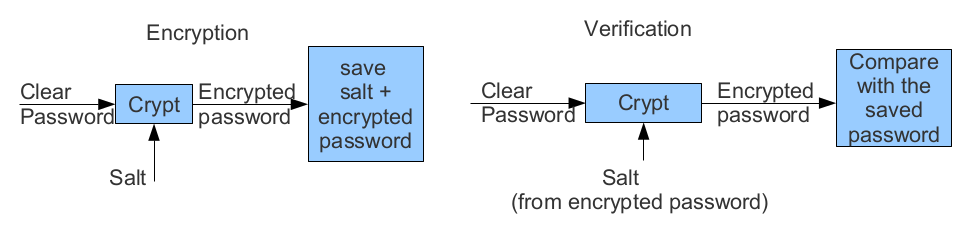
\includegraphics[scale=0.35]{chapters/7/assets/schema_o.png}
            \end{center}

        \subsubsection{Password con crypt}
            La funzione \verb|crypt()| in \textbf{glibc} itera 25 volte l'algoritmo DES per cifrare un messaggio costante (tipicamente una sequenza di 0) utilizzando una chiave simmetrica derivata dalla password in chiaro inserita dall'utente più una stringa casuale di 12 bit detta \textit{salt}.
        
            Il \textit{salt} viene scritto in chiaro all'inizio della password cifrata con codifica base64 (2 caratteri). La modifica di DES (25 iterazioni più salt) rende la cifratura non invertibile.

            La verifica della password consiste nel confronto tra i messaggi codificati: \verb|crypt| viene ripetuto con la password da verificare e il \textit{salt} prelevato dalla password cifrata. Il fatto che la cifratura non sia invertibile consente di utilizzare gli algoritmi di hashing come tecniche alternative di codifica, implementate in \textit{glibc2}.

            La funzione \verb|crypt()| in glibc2 aggiunge la possibilità di cifrare con MD5. L'hash MD5 è di 128 bit, l'output è una stringa composta al più da 34 byte di cui:
            \begin{itemize}
                \item la prima parte è il salt: \verb|$1$ <max 8 char> $|.
                \item la seconda parte è una sequenza di 22 caratteri (128 bit di MD5/6, di base 64), contenenti MD5(<salt> <clear password>).
            \end{itemize}

        \subsubsection{Comandi OpenSSL: passwd}
            Con OpenSSL è possibile generare le password utilizzando il crypt di glibc (default) oppure MD5 con l'opzione \verb|-1|.

            \verbatiminput{chapters/7/assets/schema_p.txt}

        \subsubsection{Algoritmi a chiave pubblica}
            La cifratura a chiave simmetrica ha una grave debolezza nella condivisione della chiave: il trasferimento della chiave la espone ad intercettazione.
        
            Diffie ed Hellmann (Stanford) nel 1976 proposero una tecnica nuova di crittografia, basata sull'aritmetica modulare, in cui vengono utilizzate due chiavi $K_e$ e $K_d$ distinte per la codifica $C = K_e(P)$ la decodifica $P = K_d(C)$. Assegnando ad una chiave il ruolo di "chiave privata" e all'altra il ruolo di "chiave pubblica" si supera la debolezza della chiave condivisa.

            \begin{center}
                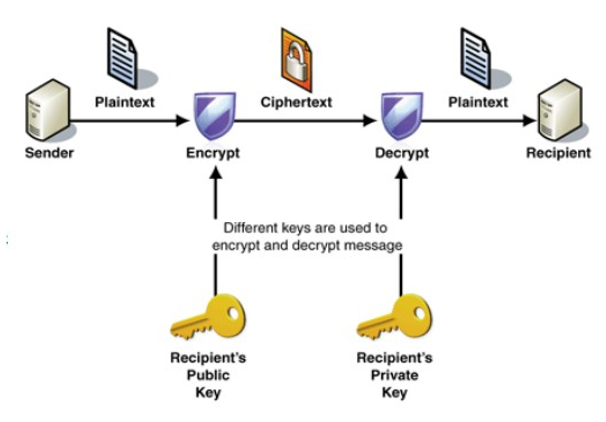
\includegraphics[scale=0.5]{chapters/7/assets/schema_q.png}
            \end{center}

            Un'importante proprietà di questo algoritmo è:
            
            \begin{equation*}
                K_d(K_e(P)) = K_e(K_d(P)) = P
            \end{equation*}

            Questo consente di poter applicare le chiave in due modi diversi ottenendo due diverse funzioni:
            \begin{itemize}
                \item Applicando prima la chiave pubblica si ottiene la \textbf{Privacy (crypt/decrypt)}.
                
                A deve inviare un messaggio $P$ riservato a B su di un canale insicuro. B possiede una coppia di chiave asimmetriche $B_e$ (privata) e $B_d$ (pubblica). A cifra $P$ con la chiave pubblica di B: $C = B_d(P)$. Solo B può decifrarlo $P = B_e(C)$
                \item Applicando prima la chiave privata si ottiene l'\textbf{Autenticazione} e l'\textbf{Inte\-grità (sign/verify)}.
                
                A deve inviare un messaggio $P$ attraverso un canale insicuro. Tutti lo possono leggere, ma chi lo riceve deve essere sicuro che è stato inviato da A.
                A possiede una coppia di chiave asimmetriche $A_e$ (privata) e $A_d$ (pubblica).
                A cifra $P$ con la propria chiave privata: $C = A_e(P)$. Chiunque può applicare la chiave pubblica di A: $P = Ae(C)$.
                La decifratura funziona solo se P è stato cifrato da A.
            \end{itemize}

        \subsubsection{RSA}
            Rivest, Shamir e Adleman del MIT implementarono nel 1978 l'algoritmo che ha preso il loro nome (\textbf{RSA}) e che è attualmente il più utilizzato nelle applicazioni crittografiche a chiave pubblica.

            L'algoritmo funziona nel seguente modo:
            \begin{enumerate}
                \item si scelgono due numeri primi casuali $p$ e $q$ sufficientemente grandi.
                \item si calcolano $m = p \cdot q$ (modulo), $z = (p - 1)(q - 1)$.
                \item si sceglie un numero $e < z$ co-primo con $z$ (senza divisori comuni)
                \item si calcola un numero $d$ tale che $e \cdot d = 1 ~ mod ~ z$
            \end{enumerate}

            Siano $(e,m)$ la chiave pubblica e $(d,m)$ la chiave privata, si ha che:

            \begin{equation*}
                C = P^e ~ mod ~ m
            \end{equation*}

            \begin{equation*}
                P = C^d ~ mod ~ m
            \end{equation*}

            Le due chiavi hanno una parte comune \textbf{m (modulo)} che è tipicamente di 1024 o 2048 bit e una parte specifica \textbf{e, d (esponenti)} di circa 20 bit.

            Per violare la chiave privata occorre determinare $d$. Questo può essere fatto solo per brute force fattorizzando $m$ che è il prodotto di due numeri primi. L'operazione richiederebbe un tempo enormemente grande anche sul più veloce dei computer. La cifratura $C = P^e ~ mod ~ m$ limita la dimensione massima di $P$ (a circa 100,200 byte, dipende dal numero di bit della chiave). Per dimensioni superiori conviene usare RSA per scambiare una chiave simmetrica.

        \subsubsection{Comandi OpenSSL: RSA}
            OpenSSL supporta RSA con i seguenti comandi: \verb|genrsa|, \verb|rsa| e \verb|rsautl|. genrsa consente di creare una coppia di chiavi RSA:

            \verb|genrsa| consente di creare una coppia di chiavi RSA:

            \verbatiminput{chapters/7/assets/schema_r.txt}

            \verb|rsa| consente di processare le chiavi RSA:

            \verbatiminput{chapters/7/assets/schema_s.txt}

            \verb|rsautl| viene utilizzato per cifrare/decifrare firmare/verificare con chiavi RSA:

            \verbatiminput{chapters/7/assets/schema_t.txt}
            
        \subsubsection{Comandi OpenSSL: Digest firmato con RSA}
            Le chiavi RSA possono essere utilizzate per firmare il digest di un messaggio: il seguente comando crea il digest di file.txt utilizzando SHA1, quindi lo firma con la chiave privata:

            \verbatiminput{chapters/7/assets/schema_u.txt}

            Per la verifica occorre il messaggio originale, il digest firmato e la chiave pubblica di chi ha firmato:

            \verbatiminput{chapters/7/assets/schema_v.txt}

        \subsubsection{Algoritmi a chiave pubblica: certificazione dell'identità}
            Se genero una coppia di chiavi, uso la chiave privata per cifrare un messaggio e pubblico il messaggio cifrato, chiunque può verificare con la mia chiave pubblica che il messaggio l'ho cifrato io, ma questo non garantisce nulla riguardo la mia identità.

            Per associare in modo certo una chiave pubblica a una persona (o host, o software) si utilizza il \textbf{certificato}, ovvero l'insieme della chiave pubblica e dei dati del proprietario firmati (cifrati con la chiave privata) da una \textbf{Autorità di Certificazione} che garantisce l'autenticità dei dati contenuti nel \textit{certificato}.

            Le applicazioni principali sono nella posta elettronica (identità del mittente), nelle conessioni web (identità del server e del client) e nel software (identità dello sviluppatore).

        \subsubsection{Certificati X.509}
            \textbf{X.509} è uno standard emanato da ITU per il formato dei certificati. Questo standard stabilisce quali informazioni possono comporre un certificato, i principali campi sono:
            \begin{itemize}
                \item \textbf{Version}: numero della versione di X.509 (v1, v2 o v3).
                \item \textbf{Serial Number}: numero univoco di emissione da parte di CA.
                \item \textbf{Signature Algorithm}: algoritmo usato per firmare il certificato.
                \item \textbf{Issuer}: Distinguished Name DN della CA che ha emesso il certificato.
                \item \textbf{Validity}: inizio e fine del periodo di validità.
                \item \textbf{Subject}: Distinguished Name DN del proprietario del certificato.
                \item \textbf{Subject Public Key Info}: chiave pubblica (modulo più esponente) ed algoritmo utilizzato.
                \item \textbf{X509v3 Extensions}: estensioni opzionali sono per v3.
                \item \textbf{Signature}: firma da parte della CA (cifrato con la chiave pubblica della
                CA).
            \end{itemize}

            \begin{center}
                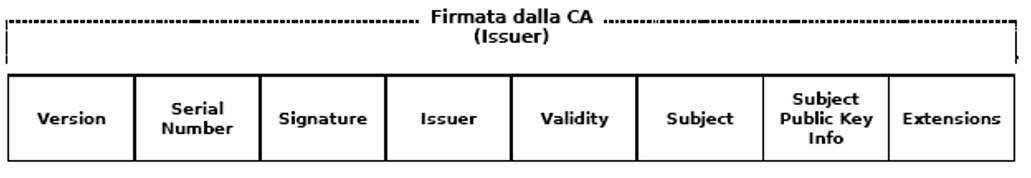
\includegraphics[scale=0.333]{chapters/7/assets/schema_w.png}
            \end{center}

        \subsubsection{La Certification Authority}
            La CA è un ente che firma le richieste di certificato da parte di una comunità di utenti/host/software garantendone l'identità.
        
            La CA possiede una propria coppia di chiavi e autofirma la propria richiesta (self-signed). Per identificare univocamente i certificati esiste un name-space gerarchico di certificati, in cui ogni nodo ha un attributo e un valore.
        
            I principali attributi sono: O (Organization), OU (Org. Unit), C (Country), CN (CommonName), etc. Ogni certificato possiede quindi un FQDN (Subject).
        
            La CA possiede un BaseDN ed è vincolata ad emettere Certificati all'interno del suo BaseDN.
        
            Una CA può firmare certificati anche per altre CA, poiché il namespace gerarchico consente di organizzare diverse CA all'interno dello stesso albero. Ogni CA deve gestire la lista dei Certificati Revocati (CRL) che va aggiornata regolarmente.

        \subsubsection{Istanze di Certification Authority}
            Alcune CA rilasciano certificati a pagamento e sono già inserite e riconosciute dai più diffusi client Web e SMTP.
        
            Generalmente una Organizzazione/Ente/Impresa può creare una CA per le certificazioni riconosciute al suo interno.
        
            Il GARR fornisce un servizio di CA per tutti gli enti afferenti:\\\verb|http://ca.garr.it/|.
        
            La CA dell'Istituto Nazionale di Fisica Nucleare (INFN):\\\verb|http://security.fi.infn.it/CA/|.
        
            TERENA (ente Europeo che integra i provider nazionali per Università ed enti di ricerca) offre un servizio di CA per i propri membri. La CA non è self-signed, ma è sotto la gerarchia DigiCert.
        
            In Italia esistono determinate Enti Certificatori Qualificati (con particolari requisiti di garanzia) che possono emettere certificati le cui firme hanno valore legale.

        \subsubsection{Comandi OpensSSL: ca}
            OpenSSL consente di creare una propria Certification Authority: questo comando genera una chiave ed un certificato autofirmato:

            \verbatiminput{chapters/7/assets/schema_x.txt}

            Con il comando \verb|ca| vengono gestite le operazioni della Certification Authority:
            \begin{itemize}
                \item Firma di una richiesta di certificato:
                
                \verb|$ openssl ca -in req.pem -out newcert.pem -config \|
                
                \verb|/var/www/html/myCA/openssl.cnf|
                \item Generazione della Certificate Revocation List:
                
                \verb|$ openssl ca -gencrl -out crl.pem|
            \end{itemize}

        \subsubsection{Comandi OpenSSL: openssl.cnf}
            Esempio di configurazione:

            \verbatiminput{chapters/7/assets/schema_y.txt}

        \subsubsection{Comandi OpenSSL: req}
            Questo comando serve per generare una richiesta di certificato.
        
            La chiave privata può essere fornita (\verb|-key|) o generata dal comando. Con l'opzione \verb|-nodes| non viene cifrata la chiave privata. Questo serve per i certificati host per i quali non è possibile digitare una passphrase.
        
            Il file di configurazione (\verb|openssl.cnf|) contiene le informazioni relative al proprietario del certificato, alcune delle quali vengono richieste interattivamente.
        
            \verbatiminput{chapters/7/assets/schema_z.txt}
        
        \subsubsection{Certificati self-signed}
            Con l'opzione \verb|-x509| non viene generata una richiesta, ma un certificato self-signed.
        
            Se il file di configurazione (\verb|-config|) non viene fornito, i dati del certificato vengono richiesti interattivamente.

            \verbatiminput{chapters/7/assets/schema_za.txt}

        \subsubsection{Formato dei certificati X.509: DER e PEM}
            I certificati X.509 possono essere rappresentati in diversi possibili formati. I principali sono: \textbf{DER}, \textbf{PEM} e \textbf{PKCS12}.
        
            \textbf{DER} è un formato binario utilizzato in ambiente Windows e Java con estensioni \verb|.der| o \verb|.cer|.
        
            \textbf{PEM} è un formato testuale (base64) ed è utilizzato prevalentemente in ambiente Unix. Può contenere certificati, richieste di certificati, chiavi private.

        \subsubsection{Comandi OpenSSl: x.509}
            Visualizzare i campi e cambiare formato (tra PEM e DER) di un certificato:

            \verbatiminput{chapters/7/assets/schema_zb.txt}

        \subsubsection{Formati dei certificati X.509: PKCS}
            \textbf{PKCS (Public Key Cryptography Standards)} è un gruppo di standard creati da RSA Data Security con lo scopo di creare formati di interoperabilità.

            Sono stati creati 15 standard, ma i formati prevalentemente utilizzati sono:
            \begin{itemize}
                \item \textbf{PKCS\#12 (Personal Information Exchange Syntax Standard)}: è nato come evoluzione di PFX, e definisce un formato per immagazzinare la chiave privata e certificato in un file protetto con password (cifratura con chiave simmetrica).
                \item \textbf{PKCS\#7 (Cryptographic Message Syntax Information)}: è un formato per rappresentare messaggi cifrati o firmati ed è utilizzato da S/MIME per l'invio di e-mail cifrate e/o firmate.
                \item \textbf{PKCS\#11 (Cryptographic Token Interface)}: definisce le API per utilizzare i token crittografici, come le SmartCard e le chiavi USB.
            \end{itemize}

        \subsubsection{Comandi OpenSSL: pkcs12}
            Questo comando serve per gestire i file in formato PKCS\#12:

            \verbatiminput{chapters/7/assets/schema_zc.txt}

        \subsubsection{Ambiente Java: keystore e keytool}
            In ambiente Java per la gestione di chiavi e certificati è spesso utilizzato il \textbf{Keystore}, la cui estensione standard è \verb|.jks| (\textbf{Java Key Store}).
        
            Ad ogni certificato nei keystore è associato un alias univoco. Il keystore è realizzato con un file protetto da password.
        
            JDK fornisce il tool \textbf{keytool} per la gestione del Keystore.
        
        \subsubsection{Firmare Software Java}
            I certificati X.509 possono essere utilizzati anche per firmare software, come ad esempio le Applet.
        
            Per firmare codice Java (in formato Jar) il comando è \verb|jarsigner|.
        
            Le chiavi per la firma possono essere contenuti il un Keystore o in un file PKCS\#12. Se utilizziamo il formato PKCS\#12 occorre estrarre il "FriendlyName" del certificato con il comando:\\
            \verb|openssl pkcs12 -info -in alfieri-sci.p12|

            È quindi possibile firmare con un comando del tipo:\\
            \verb|jarsigner -keystore alfieri-sci.p12 -storetype pkcs12 \|\\
            \verb|-signedjar applet-signed.jar applet.jar "ID di Roberto Alfieri \|\\
            \verb|a UniPRScienze"|

            Il certificato utilizzato deve essere stato abilitato dalla CA a firmare software.

        \subsubsection{Comandi OpenSSL: smime}
            \textbf{MIME (Multipurpose Internet Mail Extensions)} è una estensione del protocollo di posta elettronica per poter includere in un unico messaggio più documenti (allegati), codificati in ASCII Standard.

            MIME introduce un header in cui è possibile inserire campi che descrivono il contenuto, tra cui:
            \begin{itemize}
                \item Content-Type: tipo di dato contenuto (esempio image/JPEG).
                \item Content-transfer-encoding: codifica del contenuto (esempio base64).
            \end{itemize}

            \textbf{S/MIME (Secure/MIME)} include in questo schema, la possibilità di cifrare/decifrare il contenuto, utilizzando un algoritmo a chiave simmetrica. La chiave simmetrica viene cifrata con la chiave pubblica del destinatario e inviata insieme al messaggio stesso. (Content-Type del messaggio).

            Permette di firmare/verificare un messaggio allegando la firma (Content-Type della firma).

        \subsubsection{Cifrare/Decifrare con smime}
            Per inviare un messaggio cifrato al destinatario la chiave simmetrica viene cifrata con la chiave pubblica del destinatario e inviata assieme al messaggio stesso.
        
            Il destinatario legge la chiave simmetrica utilizzando la propria chiave privata, quindi decripta il messaggio con la chiave simmetrica.
        
            Il mittente codifica il messaggio col seguente comando:\\
            \verb|openssl smime -encrypt -text -in message.txt -out \|\\
            \verb|encrypted-message.txt dest-user-certificate.pem|

            Il Destinatario lo decodifica con il seguente comando:\\
            \verb|openssl smime -decrypt -text -in encrypted-message.txt \|\\
            \verb|-out decrypted-message.txt -inkey userkey.pem|

        \subsubsection{Firmare/Verificare con smime}
            La firma consiste nel cifrare con la chiave privata del mittente il digest del messaggio, che verrà inviato insieme al messaggio stesso.

            Si ha \textbf{garanzia dell'identità del signer} che consiste nella decifratura della firma con la chiave pubblica del \textit{signer} e si ha \textbf{garanzia di integrità del messaggio}, cioè il messaggio è integro se il digest decifrato nella firma e il digest ricalcolato sono uguali.

            Per firmare un messaggio:\\
            \verb|openssl smime -sign -text -in msg.txt  -out signed-msg.txt \|\\
            \verb|-signer usercert.pem  -inkey userkey.pem|

            Il certificato del signer è incluso nel messaggio.

            Con questo comando il destinatario estrae il certificato del signer:\\
            \verb:openssl smime -pk7out -in signed-message.txt \:\\
            \verb:| openssl pkcs7 -print_certs:

            Con questo comando il destinatario verifica il certificato del Signer tra le CA di cui si fida (\verb|-CAfile| o \verb|-CApath|), quindi usa il certificato per decifrare la firma ed estrarre il MD, infine confronta il MD ricevuto con quello calcolato:\\
            \verb|openssl smime -verify -text -in signed-msg.txt -CAfile CAcert.pem|

        \subsubsection{Creare una mail smime}
            Per spedire il messaggio occorre aggiungere le intestazioni standard: From, To, Subject.
        
            Per questo basta aggiungere al comando smime le opportune opzioni.

            \verbatiminput{chapters/7/assets/schema_zd.sh}

        \subsubsection{SSL/TLS}
            Il protocollo SSL mette in sicurezza una connessione client-server introducendo un \textbf{layer di sicurezza al livello di trasporto (TLS)}.
        
            In questo modo l'applicativo non vede più le API di TCP e deve quindi riscrivere l'interfaccia con il livello di Trasporto utilizzando le API SSL/TLS.
        
            Vengono utilizzati due protocolli principali:
            \begin{itemize}
                \item Il \textbf{Record Layer Protocol} è utilizzato per trasmettere e ricevere dati (cifratura e decifratura) mediante un cipher simmetrico.
                \item L'\textbf{Handshake Protocol} interviene solo all'inizio (o per ripristinare una sessione interrotta). Negozia i parametri per lo scambio dei dati (scambio dei certificati e condivisione di una chiave di sessione per il cipher simmetrico).
            \end{itemize}

            \begin{center}
                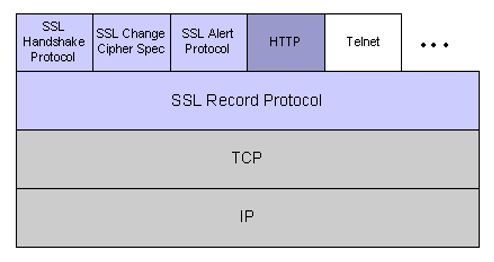
\includegraphics[scale=0.6]{chapters/7/assets/schema_ze.png}
            \end{center}

        \subsubsection{SSL Hanshake Protocol}
            \begin{enumerate}
                \item Il client manda SSL version e il cipher suite da utilizzare.
                \item Il server manda il proprio SSL versione e il cipher suite.
                \item Il server manda il proprio certificato.
                \item Il server opzionalmente richiede il certificato del client.
                \item Il client verifica il certificato del server e procede solo se è ok.
                \item Il client genera il pre-master secret.
                \item Il client cripta la chiave con il certificato del server e la invia.
                \item Se il sever ha richiesto l'autenticazione del client, il client cifra un challenge e lo invia al server.
                \item Se il server non riesce a decifrare termina la sessione.
                \item Client e server usano il pre-master secret per generare la chiave di
                sessione condivisa.
                \item Il client manda un messaggio di conclusione dell'handshake.
                \item Il server manda un messaggio di conclusione dell'handshake.                
            \end{enumerate}

            In qualsiasi momento, client e server possono rinegoziare la connessione: in questo caso si ripete la procedura.

            \begin{center}
                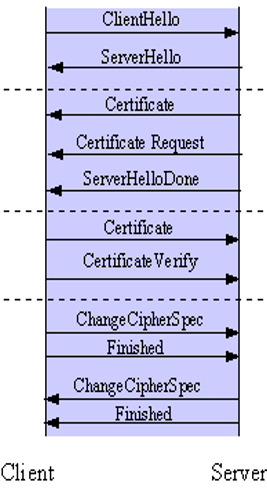
\includegraphics[scale=0.45]{chapters/7/assets/schema_zf.png}
            \end{center}

        \subsubsection{SSL Record Protocol}
            Al termine dell'Handshake Protocol inizia l'SSL Record Protocol:
            \begin{enumerate}
                \item Frammentazione del flusso.
                \item Compressione dei frammenti
                \item Calcolo del digest
                \item Cifratura
            \end{enumerate}

            \begin{center}
                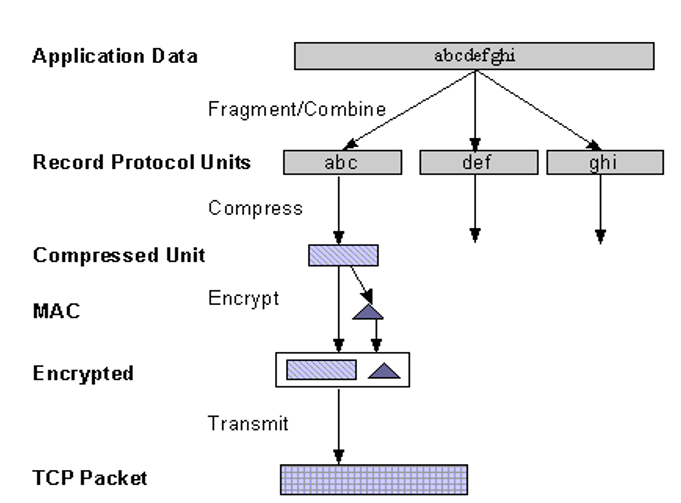
\includegraphics[scale=0.4]{chapters/7/assets/schema_zg.png}
            \end{center}

        \subsubsection{Applicazioni SSL e StartTLS}
            Le principali applicazioni SSL sono:
            \begin{itemize}
                \item \textbf{https} (HTTP over SSL) 443/tcp
                \item \textbf{pop3s} (POP3 over SSL) 995/tcp
                \item \textbf{imaps} (IMAP over SSL) 993/tcp
                \item \textbf{smtps} (SMTP over SSL) 465/tcp
                \item \textbf{ldaps} (LDAP over SSL) 636/tcp
            \end{itemize}

            \textbf{StartTLS} è un'estensione della comunicazione in chiaro, che offre l'opzione di passare ad una connessione cifrata (SSL o TLS), anziché passare ad una connessione cifrata separata.

            IMAP, SMTP, POP e LDAP hanno implementazioni con supporto StartTLS.

        \subsubsection{Comandi OpenSSL: s\_client s\_server}
            Comando s\_client:\\
            \verb|openssl s_client -connect fis.unipr.it:443 -cert usercert.pem \|\\
            \verb|-key userkey.pem -CAfile myCA.pem|

            Il client visualizza i dati della connessione, poi dal client possiamo inviare caratteri che vengono visualizzati sul server. Il carattere 'R' forza la rinegoziazione, 'Q' forza la disconnessione.

            Una volta connessi è possibile digitare manualmente i comandi da inviare al server (ad esempio, se il server è www : "GET /" e "HEAD / HTTP/1.0").

            \verbatiminput{chapters/7/assets/schema_zh.sh}

            Con l'opzione \verb|-www| emula un web server che risponde al browser con i dati salienti della connessione SSL.
            
            Comando s server:

            \verbatiminput{chapters/7/assets/schema_zi.sh}

        \subsubsection{Programmazione OpenSSL : BIO}
            La libreria SSL fornisce le API necessarie per la programmazione in C di canali cifrati. La libreria SSL fornisce una astrazione di I/O, denominata BIO, che consente di creare un canale cifrato o in chiaro.

            Per aprire un nuovo canale è necessario creare a priori un handle:

            \lstinputlisting[language=C]{chapters/7/assets/schema_zj.c}

            Per aprire una connessione senza cifratura si utilizza la chiamata \\\verb|BIO_new_connect()|:

            \lstinputlisting[language=C]{chapters/7/assets/schema_zk.c}

            È possibile verificare lo stato di una connessione con \verb|BIO_do_connect()|:

            \lstinputlisting[language=C]{chapters/7/assets/schema_zl.c}

            Per l'I/O sono disponibili \verb|BIO_read()|, \verb|BIO_write()|, \verb|BIO_puts()| e \\\verb|BIO_gets()|.

            \lstinputlisting[language=C]{chapters/7/assets/schema_zm.c}

            \verb|BIO_read()| ritorna il numero di byte letti dal canale:

            \lstinputlisting[language=C]{chapters/7/assets/schema_zn.c}

            Per chiudere la connessione si può utilizzare \verb|BIO_free_all();|

        \subsubsection{Programmazione OpenSSL: SSL CTX}
            Per creare un canale cifrato occorre gestire la struttura SSL CTX che contiene i dati (principalmente certificati e chiavi) necessari per il funzionamento di SSL.
        
            È inizializzata dalla funzione \verb|SSL_CTX_new()|:

            \lstinputlisting[language=C]{chapters/7/assets/schema_zo.c}

            La prima informazione che dobbiamo fornire è uno o più certificati di CA affidabili per le verifica dei certificati:

            \lstinputlisting[language=C]{chapters/7/assets/schema_zp.c}

            Se il client possiede una coppia di chiavi, è possibile aggiungerla al contesto:

            \lstinputlisting[language=C]{chapters/7/assets/schema_zq.c}

            Queste credenziali potrebbero essere richieste dal server.

        \subsubsection{Programmazione OpenSSL: attivazione canale sicuro}
            Il canale cifrato è attivato dalle seguenti chiamate:

            \lstinputlisting[language=C]{chapters/7/assets/schema_zr.c}

            Possiamo verificare se la connessione è attiva:

            \lstinputlisting[language=C]{chapters/7/assets/schema_zs.c}

            La struttura SSL contiene le informazioni di stato della connessione:

            \lstinputlisting[language=C]{chapters/7/assets/schema_zt.c}

            Attiviamo il modo AUTO\_RETRY (se il server chiede un nuovo handshake)

            \lstinputlisting[language=C]{chapters/7/assets/schema_zu.c}

            Verifichiamo la validità del certificato server:

            \lstinputlisting[language=C]{chapters/7/assets/schema_zv.c}

            Per chiudere il canale, oltre al \verb|BIO_free_all(bio);| dobbiamo chiudere anche il contesto \verb|SSL_CTX_free(ctx);|

        \subsubsection{Programmazione OpenSSL in Python}
            Python consente di creare connessioni SSL, sia client che server, attraverso il modulo \verb|ssl| che implementa un wrapper di TCP basato su OpenSSL.

            Esempio lato client:

            \lstinputlisting[language=Python]{chapters/7/assets/schema_zw.py}

        \subsubsection{Programmazione SSL in Java}
            Nel 1999 la SUN introdusse le \textbf{JSSE (Java Secure Sockets Extensions)}, che supportano TLS 1.0, SSL 3.0, etc.
            
            JSSE è composto dei package \verb|javax.net| e \verb|javax.net.ssl|.
        
            Per creare un socket SSL lato client invece di usare un \verb|java.net.socket|, si usa il metodo \verb|createSocket()| della classe astratta \verb|javax.net.ssl.SSLSocket| \verb|Factory|. Il socket creato con \verb|createSocket()| può essere utilizzato come un socket normale.
        
            Per creare un socket SSL lato server occorre ottenere un'istanza della classe astratta \verb|javax.net.SSLServerSocket| tramite il metodo \verb|getDefault()| di \verb|SSLServerSocketFactory|, quindi si invoca il metodo \verb|createServerSocket(| \verb|int port)| sull'oggetto ritornato.
        
            Di default, l'oggetto ritornato non supporta la crittatura (solo l'autenticazione). Per configurare e inizializzare i socket sicuri, bisogna creare un oggetto \verb|SLContext|.

    \subsection{Protocolli di Autenticazione}
        L'\textbf{Autenticazione (Authentication)}: è un servizio di sicurezza che consente di accertare l'identità dichiarata da un'entità (origine dei dati o peer in una comunicazione) mediante la verifica di credenziali.
    
        L'autenticazione può essere \textbf{mutua} oppure no, dipende dalle situazioni: ad esempio è mutua quando consulto la posta elettronica, il server si deve autenticare con me per dimostrarmi di essere il server che gestisce la mia posta. Io devo dimostrare al server che sono il titolare della mailbox.

        Le tecniche possono basarsi sulla conoscenza di un segreto (password, PIN, etc.), su tecniche crittografiche, su caratteristiche biometriche (se si tratta di una persona) quali timbro della voce, impronta digitale, fondo dell'occhio, etc.

        \subsubsection{Autenticazione tramite password}
            È un protocollo largamente utilizzato perché facile da implementare e da usare. È insicuro specialmente quando: la password non viene modificata regolarmente, le password sono individuabili con attacco al dizionario (la generazione e la verifica di un un elevato numero di possibili password, prodotte con l'ausilio di un dizionario di parole comuni). Altri svantaggi sono che la password viene trasmessa in chiaro ed i principali protocolli di autenticazione significativi sono basati su password: PAP, CHAP.

        \subsubsection{Autenticazione tramite password: PAP}
            \textbf{PAP (Password Authentication Protocol)} è un protocollo che presume che il canale sia sicuro (non intercettabile). Un client manda al server il proprio username e password, il server cerca in una tabella di nomi il nome utente e la corretteza della password applicando una funzione di tramissione (che consente di evitare che il server memorizzi la passwrod in chiaro).
        
            Questo protocollo è ancora in uso in PPP, ma è deprecato.

        \subsubsection{Autenticazione tramite password: CHAP}
            \textbf{CHAP (Challenge Handshake Authentication Protocol)} è un protocollo usato in PPP. (Windows usa una variante di CHAP detta MS-CHAP).
        
            Il server invia un numero casuale $c$ (challenge) utilizzato dal client come salt, la funzione di trasformazione $r = f(pwd,c)$ è calcolata sia dal server che dal client.
        
            L'implementazione standard di CHAP usa MD5: $r = MD5(pwd,c)$
        
            Vantaggi: la password non viene scambiata tra client e server.
        
            Problemi: il DB delle password deve essere salvato in chiaro quindi è vulnerabile ad un attacco al dizionario.
        
        \subsubsection{One-Time Password (OTP)}
            Una \textbf{OTP (One Time Password)} è una password che è valida solo per una singola sessione di accesso o una transazione, e non è quindi vulnerabile agli attacchi al dizionario.
        
            Le password sono legate tra loro secondo un determinato algoritmo e devono essere utilizzate in un ordine predefinito.
        
            Gli algoritmi che sono stati realizzati per generare OTP sono abbastanza diversi tra loro.
        
            Il più diffuso è \textbf{TOTP (Time based OTP)}: le password sono generate con unalgoritmo in funzione di una chiave segreta $k$ ed il tempo corrente $t$. Per TOTP l'algoritmo è HMAC (HOTP) in cui $Password = HMAC (t,k)$.

            Una password OTP non può essere memorizzata da una persona. Essa richiede quindi una tecnologia supplementare per poter essere utilizzata. Alcuni sistemi elettronici prevedono l'uso di speciali token che l'utente porta con sé, che generano le OTP e le mostrano utilizzando un piccolo display.

            Altri sistemi sono costituiti da un software che gira sul telefono cellulare dell'utente (Google Authenticator). In alcuni casi le OTP vengono sul lato server e le trasmettono all'utente su un canale fuori banda, come ad esempio un canale di messaggistica SMS.
        
        \subsubsection{Autenticazione con challenge e chiave simmetrica}
            Le due parti A e B che condividono una chiave simmetrica $S$, si inventano ciascuna un numero casuale, detto \textbf{challenge} ($c_1$ e $c_2$).
        
            Il server invia la propria identità (B) ed il proprio challenge ($c_1$).
        
            Il client risponde inviando la propria identità (A) e la cifratura di c1, c2 e B. Il server chiude il protocollo inviando la cifratura di c1, c2 e A.
        
            Vantaggi: i messaggi cifrati non sono esposti ad attacco al dizionario.
            
            Problemi: Se abbiamo $N$ nodi ogni nodo deve conoscere $N - 1$ chiavi.
        
        \subsubsection{Autenticazione con KDC}
            Il modello del \textbf{KDC (Key Distribution Center)} si applica ad una comunità di $N$ entità (persone/host/servizi) che devono autenticarsi reciprocamente.
        
            In questo schema ogni utente ha una singola chiave condivisa con il KDC.
        
            Esempio: A deve comunicare con B
        
            A condivide con KDC la chiave $K_a$, B condivide con KDC la chiave $K_b$.
        
            A sceglie una chiave di sessione $K_s$, invia a KDC la chiave e B, in modo cifrato. KDC decifra $K_s$ e la invia a B.
        
            \begin{equation*}
                A \rightarrow A, K_a(B,K_s) \rightarrow KDC \rightarrow K_b(A,K_s) \rightarrow B
            \end{equation*}
        
            Vantaggi: esiste una singola chiave $K_a$ per comunicare con $N$ entità.
        
            Problemi: A deve inserire la chiave $K_a$ per ogni connessione.

        \subsubsection{Autenticazione con Kerberos}
            \textbf{Kerberos} è un protocollo di autenticazione che implementa il modello KDC.

            È ampiamente diffuso soprattutto negli USA sia su Linux che Windows.

            Un sistema Kerberos gestisce una comunità di utenti (\textbf{REALM}) in cui ogni utente ha una singola chiave condivisa $K_a$ con il KDC, ma il KDC si compone di 2 server: \textbf{AS (Authentication Server)} gestisce il login, mentre \textbf{TGS (Ticket Granting Server)} gestisce la sessione.

            La password di A ($K_a$) viene usata una sola volta per tutte le autenticazioni della sessione \textbf{SSO (Single Sign On)} e rimane nel computer del client solo per pochi millisecondi.

            La chiave di sessione che A presenta a B, serve solo a dimostrare l'identità di A (autenticazione). B deciderà cosa consentire di fare ad A (autorizzazione).

            Innanzitutto A chiede all'AS la chiave di sessione $K_s$ (login sul REALM):\\
            $A \rightarrow A \rightarrow AS$\\
            $A \leftarrow K_a(Ks), K_{tgs}(A,K_s) \leftarrow AS$

            Dove $K_{tgs}$ è la chiave segreta del TGS.

            Quando A deve comunicare con B chiede al TGS un Ticket Kab da usare con B:\\
            $A \rightarrow K_{tgs}(A,K_s), B, K_s(t_1) \rightarrow TGS$\\
            $A \leftarrow K_s(B,K_{ab}), K_b(A,K_{ab}) \leftarrow TGS$

            Quindi A si rivolge a B comunicandogli la chiave di sessione $K_{ab}$:\\
            $A \rightarrow K_b(A,K_{ab}), K_{ab}(t_1) \rightarrow B$\\
            $A \leftarrow Kab(t2) \leftarrow B$

            I timestamp $t_1$ e $t_2$ impediscono che qualcuno possa intercettare i messaggi e replicarli con un mittente spoofed.
        
            \begin{center}
                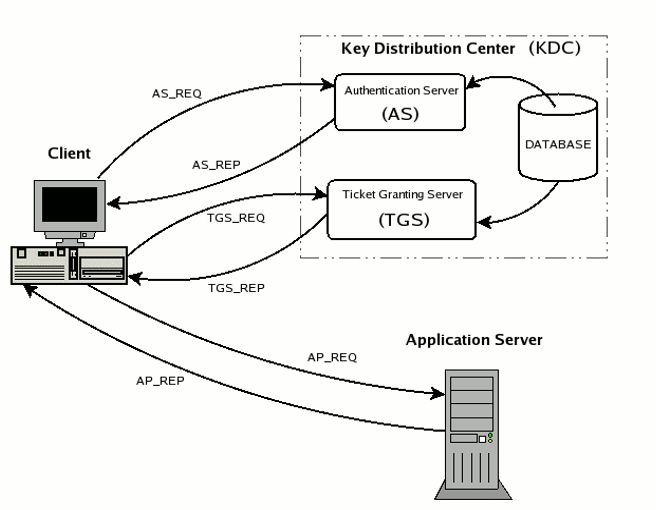
\includegraphics[scale=0.45]{chapters/7/assets/schema_zx.png}
            \end{center}

        \subsubsection{Scambio chiavi di Diffie-Hellman}
            Consente a due entità che non hanno avuto contatti in precedenza di stabilire in modo sicuro una chiave simmetrica condivisa.
        
            Offre un servizio di sicurezza di confidenzialità senza autenticazione.
        
            A e B devono condividere due numeri grandi, $n$ e $g$ che possono scambiarsi in chiaro ($n$ e $\frac{n-1}{2}$ sono numeri primi, e $g = f(n)$ è stato opportunamente calcolato).

            \begin{enumerate}
                \item A sceglie $X$ grande che mantiene segreto, quindi invia:
                
                $A \rightarrow n, g, g^X mod ~ n \rightarrow B$
                \item B sceglie $Y$ grande che mantiene segreto, quindi invia:
                
                $A \leftarrow g^Y mod ~ n \leftarrow B$
                \item B calcola $(g^X mod ~ n)^Y mod ~ n = g^{XY} mod ~ n$
                
                A calcola $(g^Y mod ~ n)^X mod ~ n = g^{XY} mod ~ n$
            \end{enumerate}

            $g^{XY}$ è la \textbf{chiave condivisa di sessione}.

        \subsubsection{Autenticazione con PKI}
            L'utilizzo di una \textbf{PKI (Public Key Infrastructure)} ha il vantaggio di non richiedere preventivamente chiavi condivise.

            I nodi A e B hanno una coppia di chiavi:

            \begin{equation*}
                A \rightarrow (E_a,D_a), B \rightarrow (E_b, D_b)
            \end{equation*}

            Le chiavi $E_a$ e $D_b$ sono pubbliche.

            A invia la propria identità e un Challenge $R_a$ a B, cifrati con la chiave pubblica di B:

            \begin{equation*}
                A \rightarrow E_b(A,R_a) \rightarrow B
            \end{equation*}

            B decifra il messaggio, sceglie una chiave di sessione $K_s$ e la invia ad A: 
            
            \begin{equation*}
                A \leftarrow E_a(R_a,R_b,K_s) \leftarrow B
            \end{equation*}

            A risponde con il challenge di B cifrato con la chiave di sessione $K_s$:
            
            \begin{equation*}
                A \rightarrow K_s(R_b) \rightarrow B
            \end{equation*}

            PKI offre i seguenti servizi di sicurezza: la chiave di sessione $K_s$ è condivisa (\textbf{confidenzialità}) e gli host hanno verificato l'identità reciproca (\textbf{autentica\-zione}).

        \subsubsection{La firma elettronica}
            La firma elettronica è l'equivalente elettronico della tradizionale firma autografa su carta.
        
            Attualmente la legge italiana prevede 4 tipologie di firma elettronica:
            \begin{itemize}
                \item Firma elettronica.
                \item Firma elettronica avanzata.
                \item Firma elettronica qualificata.
                \item Firma elettronica digitale.
            \end{itemize}

        \subsubsection{Firma Digitale}
            La \textbf{firma digitale} consente di scambiare in rete documenti con piena validità legale.
        
            La firma digitale è basata su un sistema a chiavi crittografiche asimmetriche, di cui una pubblica ed una privata, correlate tra loro di modo da consentire sia al titolare (tramite chiave privata), sia al destinatario (tramite chiave pubblica). Permette di verificare la provenienza e l'integrità del documento informatico sottoscritto digitalmente.
        
            La \textit{firma digitale} è associata ad un certificato digitale rilasciato da un soggetto con specifiche capacità professionali garantite dallo stato, viene creata mediante un dispositivo con elevate caratteristiche di sicurezza, che in genere è una smart card.
        
            Per dotarsi di firma digitale è possibile rivolgersi ai certificatori accreditati autorizzati da \textbf{AgID} che garantiscono l'identità dei soggetti che utilizzano la firma digitale.
        
            \textit{AgID} svolge attività di vigilanza sui certificatori.
        
        \subsubsection{Sistema Pubblico per la gestione dell'Identità Digitale: SPID}
            Il sistema \textbf{SPID} è costituito come insieme aperto di soggetti pubblici e privati che, previo accreditamento da parte dell'Agenzia per l'Italia Digitale, gestiscono i servizi di registrazione e di messa a disposizione delle credenziali e degli strumenti di accesso in rete nei riguardi di cittadini e imprese per conto delle pubbliche amministrazioni.
        
            Livelli di sicurezza:
            \begin{itemize}
                \item Livello 1: permette l'accesso ai servizi con nome utente e password.
                \item Livello 2: permette l'accesso ai servizi con nome utente e password insieme ad un codice temporaneo che viene inviato via SMS o con app mobile dedicata.
                \item Livello 3: permette l'accesso ai servizi con nome utente e password e l'utilizzo di un dispositivo di accesso.
            \end{itemize}

            SPID è basato sul framework \textbf{SAML (Security Assertion Markup Language)}, che permette la realizzazione di un sistema sicuro di Single Sign On (SSO) federato.

        \subsubsection{PEC: Posta Elettronica Certificata}
            La \textbf{PEC (Posta Elettronica Certificata)} permette di dare a un messaggio di posta elettronica, lo stesso valore legale di una raccomandata con avviso di ricevimento tradizionale garantendo così la prova dell'invio e della consegna.
        
            Il contenuto può essere firmato oppure criptato.
        
            L'Agenzia per l'Italia Digitale (AGID) definisce le regole tecniche e provvede al loro aggiornamento in funzione dell'evoluzione tecnologica e dell'esperienza derivante dall'utilizzo del sistema. Per la PEC devono essere usati domini dedicati (un dominio di PEC non contiene caselle e-mail non PEC).
        
            Al momento dell'invio di una mail PEC, il gestore PEC del mittente si occuperà di inviare a quest'ultimo una ricevuta che costituirà valore legale dell'avvenuta (o mancata) trasmissione del messaggio, con precisa indicazione temporale del momento in cui la mail PEC è stata inviata. In egual modo, il gestore del destinatario, dopo avergli depositato il messaggio PEC nella sua casella, fornirà al mittente una ricevuta di avvenuta consegna, con l'indicazione del momento temporale nel quale tale consegna è avvenuta.

        \subsubsection{Sicurezza nelle comunicazioni}
            La cifratura di una comunicazione può avvenire a diversi livelli.
        
            Alcune applicazioni cifrate si appoggiano sull'applicazione in chiaro. Il payload viene cifrato e quindi veicolato da applicativo non cifrato (es. S/MIME su SMTP).
        
            Il protocollo SSL/TLS fornisce un Layer intermedio tra TCP e applicazione che consente di cifrare le applicazioni. Questo richiede la riscrittura delle applicazioni che devono interfacciarsi al layer SSL anziché TCP.
        
            IPsec è un Layer di cifratura che viene posizionato a livello rete, rendendo la cifratura trasparente al livello delle applicazioni, che non devono essere modificate.
            
            L'IPsec è integrato in IPv6 (Extension Header 50 e 51), mentre è opzionale in IPv4.

            \begin{center}
                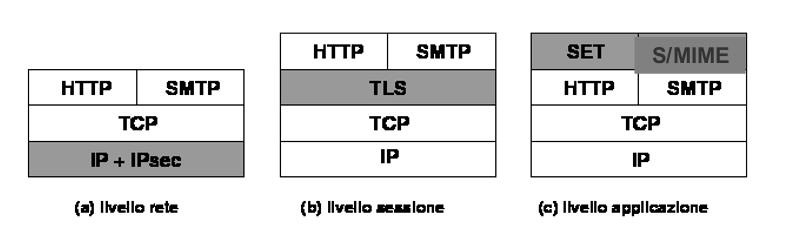
\includegraphics[scale=0.4]{chapters/7/assets/schema_zy.png}
            \end{center}

    \subsection{Protocolli IPsec}
        \textbf{IPsec}, anche se funziona a livello rete, è orientato alla connessione, a causa della cifratura con chiave. Ne consegue che le comunicazioni UDP attraverso IPsec sono poco efficienti per l'overhead elevato.
    
        Una connessione IPsec chiamata \textbf{SA (Security Association)}, è una connessione simplex e ha un identificatore di sicurezza associato. Per una connessione duplex è necessario attivare un SA per ciascuna direzione.
    
        L'identificatore, scritto in ogni pacchetto, consente al ricevente individuare la SA e quindi di reperire la chiave di decifratura.
    
        IPsec è formato da:
        \begin{itemize}
            \item Un protocollo per lo scambio delle chiavi necessarie per cifrare il canale: \textbf{IKE (Internet Key Exchange)}.
            \item Due protocolli alternativi per la cifratura dei dati sul canale: \textbf{AH (Authentication
            Header)}, gestisce l'integrità ma non la confidenzialità, \textbf{ESP (Encapsultating Security Payload)}, gestisce anche la confidenzialità tramite la cifratura del payload.
        \end{itemize}

        \subsubsection{IKE: Internet Key Exchange}
            IKE è utilizzato per stabilire una SA, è a livello applicazione e usa UDP come trasporto sulla porta 500.
        
            L'obiettivo è stabilire una \textbf{Shared Session Secret} da cui poi derivare la chiave per cifrare la SA. Viene utilizzato l'algoritmo di Diffie-Hellman.

        \subsubsection{Transport mode e Tunnel mode}
            Sia AH che ESP possono funzionare il modalità Transport o Tunnel.
            \begin{itemize}
                \item Transport mode: utilizza una connessione host-to-host, è utilizzato dagli end-point e non dai gateway. In questa modalità viene cifrato solo il payload dei datagrammi IP, e non l'header. Computazionalmente leggero. Ogni host deve avere tutto il software necessario ad implementare IPsec. Viene aggiunto solo l'header IPsec, il mittente ed il destinatario si vedono.
                \item Tunnel mode: utilizza una connessione gateway-to-gateway, è utiliz- zato per realizzare le VPN. In questa modalità viene cifrato tutto il pacchetto IP originale. Computazionalmente oneroso. Solo i gateway devono avere il software IPsec. Si hanno punti di decentralizzazione, quindi single point of failure. Si ha un doppio incapsulamento, aggiungendo l'header del gateway e l'header IPsec.
            \end{itemize}

        \subsubsection{AH: Authentication Header}
            \textbf{AH (Authentication Header)} gestisce l'integrità del pacchetto, ma non la confidenzialità: non ha la cifratura.
        
            Il protocollo determina una intestazione di 24 Byte che contiene l'HMAC del Datagramma IP (Header e payload).
        
            L'intestazione che può essere inserita nelle estensioni dei protocolli IPv4 e IPv6 (Transport Mode), oppure nell'estensione di un nuova intestazione IP che come payload incapsula il pacchetto IP originale (Tunnel Mode).

            \begin{center}
                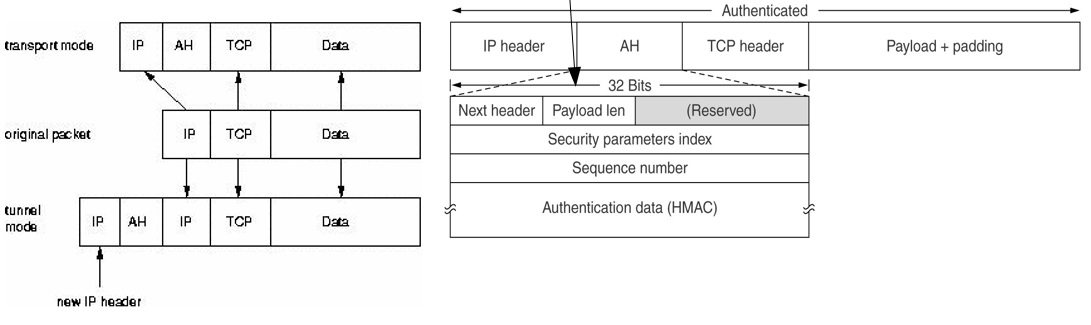
\includegraphics[scale=0.31]{chapters/7/assets/schema_zz.png}
            \end{center}

        \subsubsection{ESP: Encapsulating Security Payload}
            \textbf{ESP (Encapsulating Security Payload)} rispetto a HA, aggiunge la confidenzialità poich è il payload che viene cifrato.
        
            Viene aggiunto un nuovo campo HMAC (diversamente da AH) che non copre l'header IP. HMAC è accodato al payload cifrato. Viene calcolato mentre il pacchetto sta uscendo.
        
            La cifratura può essere:
            \begin{itemize}
                \item Transport: viene cifrata la trama di trasporto (TCP Header e payload).
                \item Tunnel: viene cifrato il pacchetto IP (IP header, TCP header e payload).
            \end{itemize}

            \begin{center}
                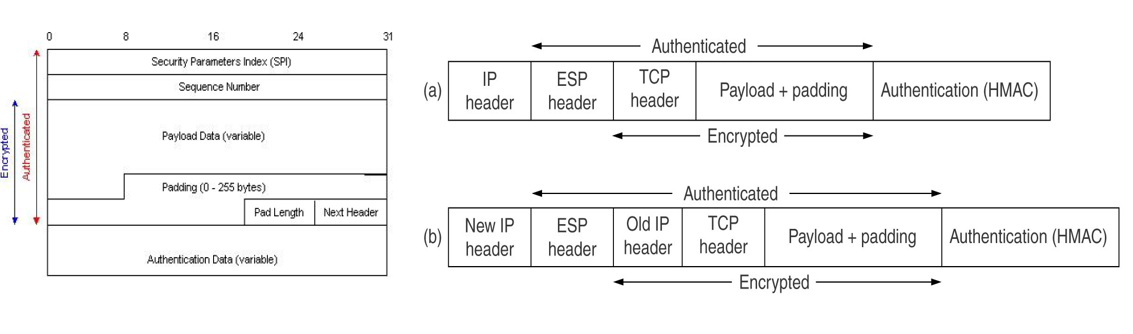
\includegraphics[scale=0.3]{chapters/7/assets/schema_zza.png}
            \end{center}

    \subsection{VPN}
        Una \textbf{VPN (Virtual Private Network)} è una rete privata instaurata tra soggetti che utilizzano un mezzo di trasmissione pubblico e condiviso come ATM o, più frequentemente, Internet.
    
        L'utilizzo tipico in Internet è tra due o più LAN remote oppure tra una LAN e un singolo host. (ad esempio, una persona che si trova all'esterno della propria struttura e vuole connettere il proprio portatile come se fosse all'interno). In entrambi i casi viene generato un tunnel protetto tra due gateway.
    
        I protocolli più utilizzati per realizzare il tunnel cifrati sono:
        \begin{itemize}
            \item IPsec, SSL/TLS, PPTP (Point-to-Point Tunnelling Protocol di Microsoft).
            \item L2TP (Layer 2 Tunnelling Protocol) e L2TPv3.
        \end{itemize}

    \subsection{Sicurezza WiFi}
        \subsubsection{WEP}
            I collegamenti wireless sono particolarmente esposti ad attacchi alla sicurezza per mancanza di barriere fisiche. \textbf{WEP (Wired Equivalent Privacy)} è stato il primo algoritmo di cifratura (1999) utilizzato per proteggere le comunicazioni Wifi (802.11).

            WEP utilizza RC4 con chiavi a 40 o 104 bit, combinate con un \textbf{Vettore di Inizializzazione (IV)} di 24 bit che viene spedito in chiaro assieme al testo cifrato (simile al salt).

            Il protocollo WEP ha dei problemi: la chiave è condivisa, quindi è violabile, il CRC non è sicuro: è possibile modificare il messaggio mantenendo coerente il CRC, anche senza conoscere la chiave.

            \begin{center}
                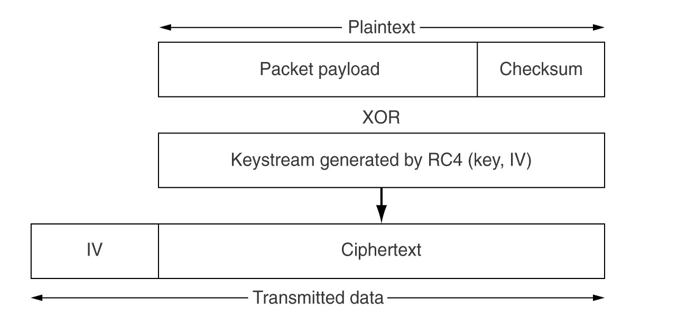
\includegraphics[scale=0.4]{chapters/7/assets/schema_zzb.png}
            \end{center}

        \subsubsection{WPA e 802.11i}
            Per superare la debolezza della cifratura WEP, il Working Group 802.11 ha ratificato nel 2004 un nuovo standard di sicurezza per 802.11 denominato \textbf{802.11i}, che rappresenta una estensione di WEP.
        
            In attesa di 802.11i la "WiFi Alliance" (il gruppo che gestisce lo standard WiFi) aveva sviluppato il protocollo \textbf{WPA (WiFi Protected Access)} che supporta parzialmente 802.11i. WiFi Alliance ha invece denominato \textbf{WPA2} il nuovo protocollo 802.11i.
        
            Cifratura: WPA, come WEP, utilizza la cifratura simmetrica RC4, mentre WPA2 utilizza AES, ma la chiave oltre che Pre-Shared (PSK) può essere cambiata dinamicamente con il protocollo \textbf{TKIP (Temporal Key Integrity Protocol)}.
        
            Autenticazione: WPA è progettato per utilizzare lo standard \textbf{IEEE 802.1x} per gestire l'autenticazione dei client e dei server e la distribuzione di differenti chiavi per ogni utente.
        
        \subsubsection{IEEE-801.X}
            È uno standard per autenticare e autorizzare l'accesso alla rete (LAN, MAN, WiFi) stabilendo una connessione punto-punto cifrata tra \textbf{Supplicant} (client) e \textbf{Authenticator} (Access Point Wifi, Switch, etc.).
        
            Generalmente l'Authenticator si rivolge ad un \textbf{Authentication Server} (ad esempio, server Radius).
        
            Quando il \textit{Supplicant} chiede l'accesso alla rete, deve prima autenticarsi all'\textit{Authenticator} (Access Point) mediante il protocollo \textbf{EAP (Extensible Authentication Protocol)}.
        
            L'autenticatore reincapsula EAP nel protocollo \textbf{RADIUS} utilizzato per la comunicazione tra Access Point e l'Authentication Server (Radius server).

        \subsubsection{Protocolli EAP e RADIUS}
            \textbf{EAP (Extensible Authentication Protocol)} è un protocollo che estende le funzionalità di Point-to-Point Protocol (PPP) consentendo l'utilizzo di diversi metodi di autenticazione (kerberos, chiave pubblica, smart card, one-time password, etc.) gestiti sotto forma di modulo plug-in.
        
            I metodi di autenticazione EAP sono:
            \begin{itemize}
                \item \textbf{EAP-TLS}: Usa TLS per la mutua autenticazione. Sia il server Radius che il Supplicant devono avere un certificato X.509.
                \item \textbf{EAP-TTLS (Tunneled TLS)}: ll vantaggio di questi metodi è che solo il server Radius deve disporre di un certificato server e della chiave privata. Funziona in due passaggi:
                \begin{enumerate}
                    \item Un algoritmo asimmetrico basato sulle chiavi del server è utilizzato per verificare l'identità del server e per creare il tunnel di cifratura simmetrica.
                    \item Il tunnel cifrato è utilizzato per trasferire username a password, utilizzando un ulteriore protocollo, dopo di ché il tunnel è abbattuto.
                \end{enumerate}
                \item \textbf{EAP-LEAP}: Soluzione proprietaria Cisco.
            \end{itemize}

            \textbf{RADIUS} è un protocollo \textbf{AAA (Autenticazione, Autorizzazione e Accounting)} utilizzato per l'accesso alla rete Internet.

        \subsubsection{Sicurezza del DNS: DNSSEC}
            Le \textbf{DNSSEC (Domain Name System Security Extensions)} sono una serie di specifiche dell'IETF per garantire la sicurezza e l'affidabilità delle informazioni fornite dai sistemi DNS.

            Ogni zona è dotata di una coppia di chiavi pubblica/privata. La chiave privata di una zona, firma singoli dati DNS in quella zona, creando firme digitali che vengono anche pubblicate con il sistema DNS.

            Quando un utente desidera accedere ad un sito web, uno stub resolver all'interno del sistema operativo dell’utente, richiede la registrazione del nome di dominio da un server del nome ricorsivo, situato presso un ISP. Dopo che il server ha richiesto questo record, richiede anche la chiave DNSSEC associata alla zona. Questa chiave consente al server di verificare che le informazioni ricevute siano identiche al record presente sul server del nome autoritativo.